\documentclass{article}
\usepackage[utf8]{inputenc}
\newcommand{\ii}{{\bf i}}
\newcommand{\jj}{{\bf j}}
\newcommand{\kk}{{\bf k}}
\newcommand{\id}{{\bf 1}}
\newcommand{\hur}{\frac{\id+\ii+\jj+\kk}{2}}%The "Hurwitz point"
\newcommand{\hurwitz}{\Z\left[\hur,\ii,\jj,\kk\right]}%The set of Hurwitz integers
\usepackage{wrapfig}
\usepackage{calligra}
\usepackage[utf8]{inputenc}
\usepackage[dvips]{graphicx}
\usepackage{a4wide}
\usepackage{amsmath}
\usepackage{mathtools}
\usepackage{euscript}
\usepackage{amssymb}
\usepackage{amsthm}
\usepackage{amsopn}
\usepackage[colorinlistoftodos]{todonotes}
\usepackage{graphicx}
\usepackage[T1]{fontenc}
\newcommand\mybar{\kern1pt\rule[-\dp\strutbox]{.8pt}{\baselineskip}\kern1pt}

\usepackage{ulem}
\usepackage{xcolor}
\newcommand{\cs}[1]{\color{blue}{#1}\normalcolor}

%Matrix commands
\newcommand{\ba}{\begin{array}}
\newcommand{\ea}{\end{array}}
\newcommand{\bmat}{\left[\begin{array}}
\newcommand{\emat}{\end{array}\right]}
\newcommand{\bdet}{\left|\begin{array}}
\newcommand{\edet}{\end{array}\right|}
\newcommand{\inv}[1]{#1^{-1}}

%Environment commands
\newcommand{\be}{\begin{enumerate}}
\newcommand{\ee}{\end{enumerate}}
\newcommand{\bi}{\begin{itemize}}
\newcommand{\ei}{\end{itemize}}
\newcommand{\bt}{\begin{thm}}
\newcommand{\et}{\end{thm}}
\newcommand{\bp}{\begin{proof}}
\newcommand{\ep}{\end{proof}}
\newcommand{\bprop}{\begin{prop}}
\newcommand{\eprop}{\end{prop}}
\newcommand{\bl}{\begin{lemma}}
\newcommand{\el}{\end{lemma}}
\newcommand{\bc}{\begin{cor}}
\newcommand{\ec}{\end{cor}}
\newcommand{\lcm}{\mbox{lcm}}
\newcommand{\defn}{\fbox{definition}}
\newcommand{\prop}{\fbox{proposition}}
\newcommand{\stab}{\mbox{stab}}
\newcommand{\Aut}{\mbox{Aut}}
\newcommand{\orb}{\mbox{orb}}

\newcommand{\norm}{\righttriangle}

\newcommand{\and}{\wedge}
\newcommand{\or}{\vee}

%sets of numbers
\newcommand{\N}{\mathbb{N}}
\newcommand{\Z}{\mathbb{Z}}
\newcommand{\Q}{\mathbb{Q}}
\newcommand{\R}{\mathbb{R}}

\newcommand{\topT}{\mathcal{T}}
\newcommand{\standtop}{\mathcal{T}_{STD}}
\newcommand{\cc}{\mathcal{C}}


\documentclass{article}
\usepackage[utf8]{inputenc}
\newcommand{\ii}{{\bf i}}
\newcommand{\jj}{{\bf j}}
\newcommand{\kk}{{\bf k}}
\newcommand{\id}{{\bf 1}}
\newcommand{\hur}{\frac{\id+\ii+\jj+\kk}{2}}%The "Hurwitz point"
\newcommand{\hurwitz}{\Z\left[\hur,\ii,\jj,\kk\right]}%The set of Hurwitz integers
\usepackage{wrapfig}
\usepackage{calligra}
\usepackage[utf8]{inputenc}
\usepackage[dvips]{graphicx}
\usepackage{a4wide}
\usepackage{amsmath}
\usepackage{euscript}
\usepackage{amssymb}
\usepackage{amsthm}
\usepackage{amsopn}
\usepackage[colorinlistoftodos]{todonotes}
\usepackage{graphicx}
\usepackage[T1]{fontenc}
\newcommand\mybar{\kern1pt\rule[-\dp\strutbox]{.8pt}{\baselineskip}\kern1pt}

\usepackage{ulem}
\usepackage{xcolor}

\newcommand{\cs}[1]{\color{blue}{#1}\normalcolor}

%Matrix commands
\newcommand{\ba}{\begin{array}}
\newcommand{\ea}{\end{array}}
\newcommand{\bmat}{\left[\begin{array}}
\newcommand{\emat}{\end{array}\right]}
\newcommand{\bdet}{\left|\begin{array}}
\newcommand{\edet}{\end{array}\right|}
\newcommand{\inv}[1]{#1^{-1}}

%Environment commands
\newcommand{\be}{\begin{enumerate}}
\newcommand{\ee}{\end{enumerate}}
\newcommand{\bi}{\begin{itemize}}
\newcommand{\ei}{\end{itemize}}
\newcommand{\bt}{\begin{thm}}
\newcommand{\et}{\end{thm}}
\newcommand{\bp}{\begin{proof}}
\newcommand{\ep}{\end{proof}}
\newcommand{\bprop}{\begin{prop}}
\newcommand{\eprop}{\end{prop}}
\newcommand{\bl}{\begin{lemma}}
\newcommand{\el}{\end{lemma}}
\newcommand{\bc}{\begin{cor}}
\newcommand{\ec}{\end{cor}}
\newcommand{\lcm}{\mbox{lcm}}
\newcommand{\defn}{\fbox{definition}}
\newcommand{\prop}{\fbox{proposition}}
\newcommand{\stab}{\mbox{stab}}
\newcommand{\Aut}{\mbox{Aut}}
\newcommand{\orb}{\mbox{orb}}

\newcommand{\norm}{\righttriangle}

\newcommand{\and}{\wedge}
\newcommand{\or}{\vee}



%sets of numbers
\newcommand{\N}{\mathbb{N}}
\newcommand{\Z}{\mathbb{Z}}
\newcommand{\Q}{\mathbb{Q}}
\newcommand{\R}{\mathbb{R}}
\newcommand{\TT}{\mathbb{T}^2}
\newcommand{\RPT}{\mathbb{RP}^2}
\newcommand{\ST}{\mathbb{S}^2}

\newcommand{\topT}{\mathcal{T}}
\newcommand{\standtop}{\mathcal{T}_{STD}}
\newcommand{\cc}{\mathcal{C}}


\title{Topology}
\author{August bergquist}


\begin{document}

\maketitle

\fbox{Theorem 12.23} If $X$ and $Y$ are topological spaces, and $f$ is a map $X\rightarrow Y$, then the induced "homomorphism" $f_*$ is well defined, and actually is a homomorphism.\\

\fbox{proof} First, suppose that $\alpha$ and $\beta$ are homotopic loops in $X$ based at $x_0$, that is, $[\alpha] = [\beta]$. We will show that the images of $[\alpha]$ and $[\beta]$ are equal. In other words, that $f_*([\alpha]) = f_*([\beta])$. Or, as is equivalent from the definition of $f_*$, that $[f\circ \alpha] = [f\circ \beta]$.\\

Let's first verify $f_*([\alpha]) = [f\circ\alpha]\in \pi_1(Y, f(x_0))$ and $f_*([\beta]) = [f\circ \beta]\in \pi_1(Y, f(x_0))$. This amounts to showing that $f\circ \alpha$ and are is actually a loops based at $f(x_0)$ Otherwise the codomain of $f$ is not even what it is claimed to be.\\

Since $\alpha$ and $\beta$ are arbitrary, it suffices to show thtat $[f\circ \alpha]\in \pi_1(Y, f(x_0))$. Since $f$ is a function from $X$ to $Y$, and $\alpha$ is a function from $[0,1]$ to $X$, it follows that the composition $f\circ\alpha$ is well defined. Furthermore, $f$ is continuous from $X$ to $Y$, and $\alpha$ is continuous from $[0,1]$ to $X$, and the composition of continuous functions is continuous, hence $f\circ \alpha$ is a continuous function from $[0,1]$ to $Y$. \\

It remains to be shown that $f\circ \alpha(0) = f\circ \alpha(1) = f(x_0)$. By composition, and since $\alpha(0) = x_0$, it follows that $f\cric\alpha(0) = f(\alpha(0)) = f(x_0)$. Similarly, by composition and since $\alpha(1) = x_0$, it follows that $f\circ \alpha(1) = f(\alpha(1)) = f(x_0)$.\\

We have verified that $f\circ\alpha$ really is a loop in $Y$ based at $f(x_0)$, and hence that $f_*([\alpha]) = [f\circ \alpha]\in \pi_1(X,x_0)$. Since $\alpha$ was arbitrary, all elements of $\pi_1(X,x_0)$ are maped to something in $\pi_1(Y, f(x_0))$ under $f_*$, hence the codomain of $f_*$ is as advertised.\\

Having shown that $f_*([\alpha])$ and $f_*(\beta)$ really are elements of $\pi_1(Y, f(x_0))$, and since path equivalence is an equivalence relation, it follows that in proving that $f_*([\alpha]) = [f\circ \alpha] = f_*([\beta]) = [f\circ \beta]$, it suffices to show that $f\circ \alpha \sim f\circ \beta$. To show this, we must find a homotopy. \\

Since $\alpha\sim \beta$ in $X$, there must exist some homotopy from $\alpha$ to $\beta$. Call this homotopy $H: [0,1]\times[0,1]\rightarrow X$. Consider the function $F$ defined $F 
= f\circ H : [0,1]\times [0,1]\rightarrow Y$. We will show that $F$ is in fact a homotopy between $f\circ \alpha$ and $f\circ \beta$, and hence $f\circ\alpha\sim f\circ \beta$, and thus by transitivity of equivalence relations $[f\circ \alpha] = [f\circ \beta]$ (that is, $f_*([\alpha]) = f_*([\beta])$). This turns out to be fairly straightforward:
\begin{enumerate}
    \item Since by definition of a homotopy, $H(s, 0) = \alpha(s)$ for all $s\in [0,1]$, it follows that $F(s,0) = f\circ H(s,0) = f(H(s,0)) = f(\alpha(s)) = f\circ \alpha(s)$ for all $s\in [0,1]$. This satisfies the first requirement.
    \item Since by definition of a homotopy, $H(s,1) = \beta(s)$ for all $s\in [0,1]$, it follows that $F(s, 1) = f\circ H(s,1) = f(H(s,1)) = f(\beta(s)) = f\circ \beta(s)$ for all $s\in [0,1]$. This satisfies the second requirement.
    \item Since by definition of a homotopy, $H(0,t) = \alpha(0) = \beta(0)$ for all $t\in [0,1]$, it follows by construction of $F$ that $F(0,t) = f\circ H(0,t) = f(H(0,t))$. Hence by substitution $F(0,t) = f(\alpha(0)) = f\circ \alpha(0) = f(x_0) = f\circ \beta(0)$ (since $f\circ \alpha$ and $f\circ \beta$) are loops in $Y$ based at $f(x_0)$, as we have shown in the first part of this proof.) This satisfies the third requirement.
    \item Finally, since by definition of a homotopy, $H(1,t) = \alpha(1) = \beta(1) = x_0$ for all $t\in [0,1]$, it follows by construction of $F$ that $F(1,t) = f\circ H(1,t) = f(H(1,t)) = f(x_0) = \alpha(1) = \beta(1)$ for all $t\in [0,1]$.  This satisfies the fourth requirement.
\end{enumerate}
Having shown that all of the requirements are met, we conclude that $F$ is a homotopy from $f\circ\alpha$ to $f\circ \beta$. Hence $f\circ \alpha\sim f\circ \beta$, and $f_*([\alpha]) = [f\circ \alpha] = [f\circ \beta] = f_*([\beta])$. Hence $f_*$ is well defined.\\

Now we must show that $f_*$ is a group homomorphism from $\pi_1(X,x_0)$ to $\pi_1(Y,f(x_0)).$ That is, we must show that for all two equivalence classes $[\alpha],[\beta]\in \pi_1(X,x_0) $, $f_*([\alpha]\cdot[\beta]) = f_*([\alpha])\cdot f_*(\beta)$. Since by the operation defined on the fundamental group $[\alpha]\cdot[\beta] = [\alpha\cdot\beta]$, and by substitution and applying the definition of $f_*$, it suffices to show that $[f\circ(\alpha\cdot\beta)] = [(f\circ \alpha)\cdot (f\circ \beta)].$ Since equivalence relations are transitive, this amounts to showing that for any loops $\alpha$ and $\beta$ in $X$ based at $x_0$, the $f\circ (\alpha\cdot \beta)\sim (f\circ \alpha)\cdot (f\circ \beta)$.
Our proof reduces to demonstrating the equivalence of these loops.
\\


Unfortunately, this follows pretty much directly from the definition of concatenation and function composition. This can be seen by repeatedly invoking these definitions:

\begin{align}
    f\circ(\alpha\cdot\beta)(s) = f(\alpha\cdot\beta(s)) = f\Bigg(\begin{dcases}
    \alpha(2s) & 0\le s \le \frac{1}{2}\\
    \beta(2s-1) & \frac{1}{2} \le s \le 1
    \end{dcases}
    \Bigg)\\
    = 
    \begin{dcases}
    f(\alpha(2s)) & 0\le s \le \frac{1}{2}\\
    f(\beta(2s-1)) & \frac{1}{2} \le s \le 1
    \end{dcases} = 
    \begin{dcases}
    f\circ \alpha(2s) & 0\le s \le \frac{1}{2}\\
    f\circ \beta(2s-1) & \frac{1}{2} \le s \le 1
    \end{dcases} = (f\circ\alpha)\cdot(f\circ \beta)(s)
\end{align}
for all $s\in [0,1]$. Since $f\circ(\alpha\cdot\beta)$ and $(f\circ\alpha)\cdot (f\circ\beta)$ agree for all $s$ in their shared domain $[0,1]$, and since their codomains and domains are the same, it follows that $f\circ(\alpha\cdot\beta) = (f\circ\alpha)\cdot (f\circ\beta)$. We have already shown that path equivalence is an equivalence relation, and equivalence relations are necessarily reflexive, hence $f\circ(\alpha\cdot\beta) \sim (f\circ\alpha)\cdot (f\circ\beta)$. Since the proof of $f_*$ as a homomorphism reduced to proving this proposition, this concludes the proof. \\

Q.E.D.
\\



\fbox{definition} Let $X$ and $ion that Y$ be topological spaces, and let $f,g:X\rightarrow Y$ be maps. We say that $f$ and $g$ are \textbf{homotopic}, and write $f\simeq g$, whenever there is a map $F:X\times [0,1]\rightarrow Y$ satisfying 
\begin{itemize}
    \item $F(x,0) = f(x)$ for all $x\in X$,
    \item $F(x,1) = g(x)$ for all $x\in X$.
\end{itemize}
In this case we call the map $F$ a homotopy from $f$ to $g$.\\

\fbox{definition} Two spaces $X$ and $Y$ are \textbf{homotopy equivalent} if there exists continuous maps $f:X\rightarrow Y$ and $g:Y\rightarrow X$ such that $g\circ f \simeq id_X$ and $f\circ g \simeq id_Y$.\\

\fbox{A Lemma for the Lemma: the Metalema} Let $X$, $Y$ and $Z$ be topological spaces, and let $f,f':X\rightarrow Y$ and $g,g':Y\rightarrow Z$ be maps such that $f\simeq f'$ and $g\simeq g'$. Then it follows that $f\circ g\simeq f'\circ g'$. 
\\
\fbox{proof} To prove the Metalema, we must construct a map $H:X\times [0,1]\rightarrow Z$ such that (1) $H(x,0) = f\circ g(x)$ and (2) $H(x,1) = f'\circ g'(x)$ for all $x\in X$.\\
Since $f\simeq f'$ there exists a homotopy $F:X\times[0,1]\rightarrow Y$ from $f$ to $f'$. Moreover, since $g\simeq g'$ there exists a homotopy $G:Y\times [0,1]\rightarrow Z$ from $g$ to $g'$. Consider the function $H:X\times[0,1]\rightarrow Z$ defined $H(x,t) = F(G(x,t),t)$ (note that this is not quite a composition since the domains and codomains do not match up, though it certainly resembles one).  \\

I'm not sure how to rigorously prove the continuity of $H$. it is annoyingly close to a composition. It would involve something to do with the product topology, so I will simply take for granted that $H$ is a continuous function from $[0,1]^2$ to $Z$. \\

Let $x$ be arbitrary in $X$. To verify the other requirements of a homotopy, observe that $H(x,0) = F(G(x,0),0) = F(g(x),0) = f(g(x)) = f\circ g(x)$, where we have used the fact that $F$ is a homotopy from $f$ to $f'$, and $g$ to $g'$. Similarly, using the same facts, we have $H(x,1) = F(G(x,1),1) = F(g'(x),1) = f'(g'(x)) = f'\circ g'(x)$.\\

Since $x$ was arbitary in $X$, it follows that for all $x\in X$, (1) $H(x,0) = f\circ g(x)$ and (2) $H(x,1) = f'\circ g'(x)$. Hence the two requirements of a homotopy (other than continuity, which we are taking for granted) are satisfied. This verifies that $H$ is a homotopy from $f\circ g$ to $f'\circ g'$, hence $f\circ g\simeq f'\circ g'$ whenever $f\circ f'$ and $g\circ g'$. 
\\


\fbox{Lemma 12.28} Homotopy equivalence of spaces is an equivalence relation. 

\fbox{proof} Let $X$, $Y$, and $Z$ be topological spaces.
\begin{itemize}
    \item First, we must verify reflexivity holds for the homotopy "equivalence" relation. That is, we must show that $X$ is homotopy equivalent to itself. This is fairly straightorward: consider $f = id_X : X\rightarrow X$ and $g = id_X: X \rightarrow X$. The fact that $f$ and $g$ are continuous follows directly from the fact that the identity map is continuous. Moreover, observe that $f\circ g = id_X\circ id_X = id_X$. Consider the function $F:X\times [0,1]\rightarrow X$ defined $F(x,t) = x$ for all $(x,t)\in X\times [0,1]$.  
    \item Now we must verify that symmetry holds. This follows easily, as the definition of homotopy equivalence is itself symmetric (in that the naming of $f$ and $g$ are named arbitrarily). 
    \item The interesting part is transitivity. Suppose that $X$ is homotopy equivalent to $Y$, and that $Y$ is homotopy equivalent to $Z$. We must show that $X$ is homotopy equivalent to $Z$. \\
    
    Since $X$ is homotopy equivalent to $Y$, there exists maps $f:X\rightarrow Y$ and $g:Y\rightarrow X$ which satisfy $g\circ f\simeq id_X$ and $f\circ g\simeq id_Y$. Moreover, since $Y$ is homotopy equivalent to $Z$, there exists functions $f':Y\rightarrow Z$ and $g':Z\rightarrow Y$ such that $g'\circ f' \simeq id_Y$ and $f'\circ g'\simeq id_Z$. Consider the functions $f'\circ f: X\rightarrow Z$ and $g\circ g':Z\rightarrow X$. We will show that these functions are homotopy equivalences.\\
    
    First, consider the composition $(f'\circ f)\circ (g\circ g')$. Since function composition is  associative, $(f'\circ f)\circ (g\circ g') = f'\circ(f\circ g)\circ g'$. Moreover, since $f\circ g\simeq id_Y$, it follows by the Metalemma that $f'\circ(f\circ g) \simeq f\circ id_Y$. Since $f'\circ id_Y = f$ (recall this result from foundations), and since by Theorem 12.5 we know that homotopy of continuous functions is an equivalence relation, and hence reflexive, it follows that $f'\simeq f'\circ id_Y$, hence by the Metalemma $f'\circ (f\circ g) \simeq f'\circ id_Y$. Since homotopy is an equivalence relation, it is transitive, hence $f\circ(f\circ g)\simeq $
\end{itemize}
\begin{figure}
    \centering
    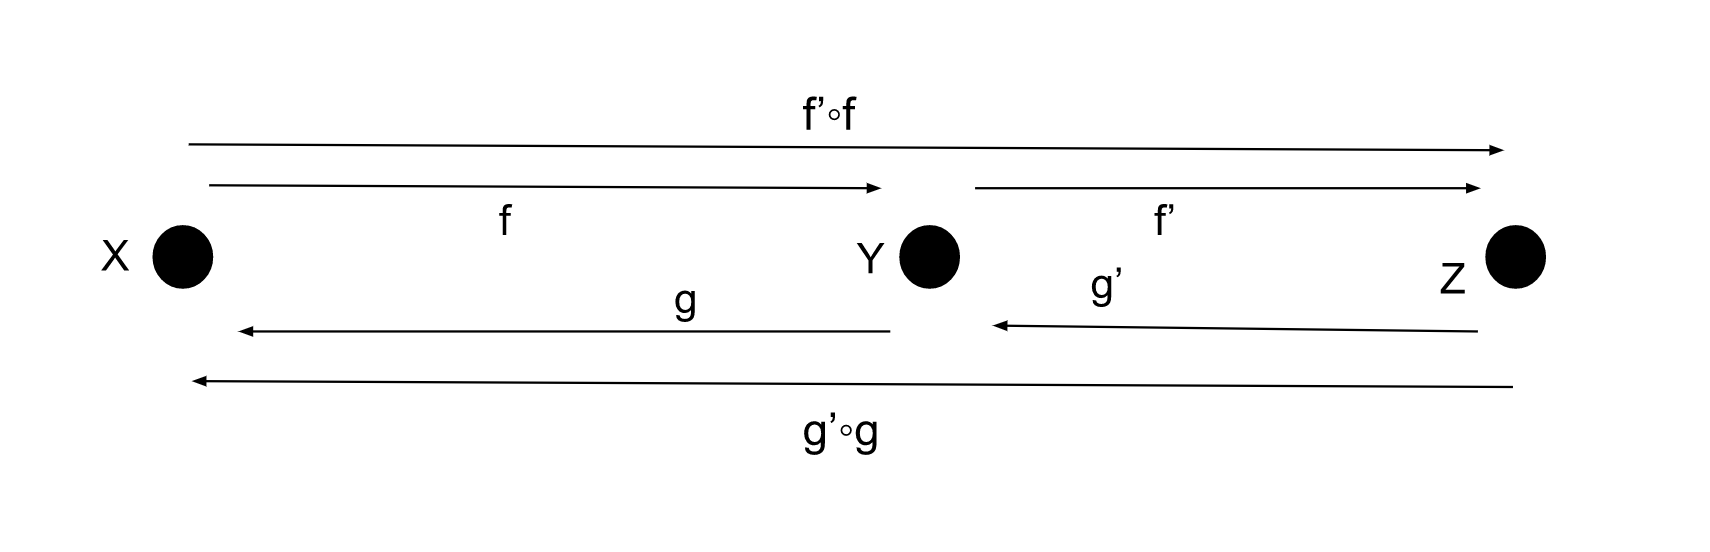
\includegraphics{functions.png}
    \caption{Caption}
    \label{fig:my_label}
\end{figure}
\end{document}